\que{Выпуклые множества. Надграфик функции, критерий выпуклости функции (с доказательством).}

Выпуклые множества -- см. \textbf{\hyperref[выпуклое множество]{Определение \ref{выпуклое множество}}}.

\begin{multicols}{2}
\begin{definition}[Надграфик функции]
	Надграфиком функции $f(x)$, определенной на множестве $U\in E^n$, называется множество (см. Рисунок \ref{fig:teor9})
	\begin{equation*}
		\operatorname{epi} f = \left\{ (x,y)\in E^{n+1}:\: x\in U,\,y\geq f(x) \right\}
	\end{equation*}
	\columnbreak
	\begin{figure}[H]
	\centering
	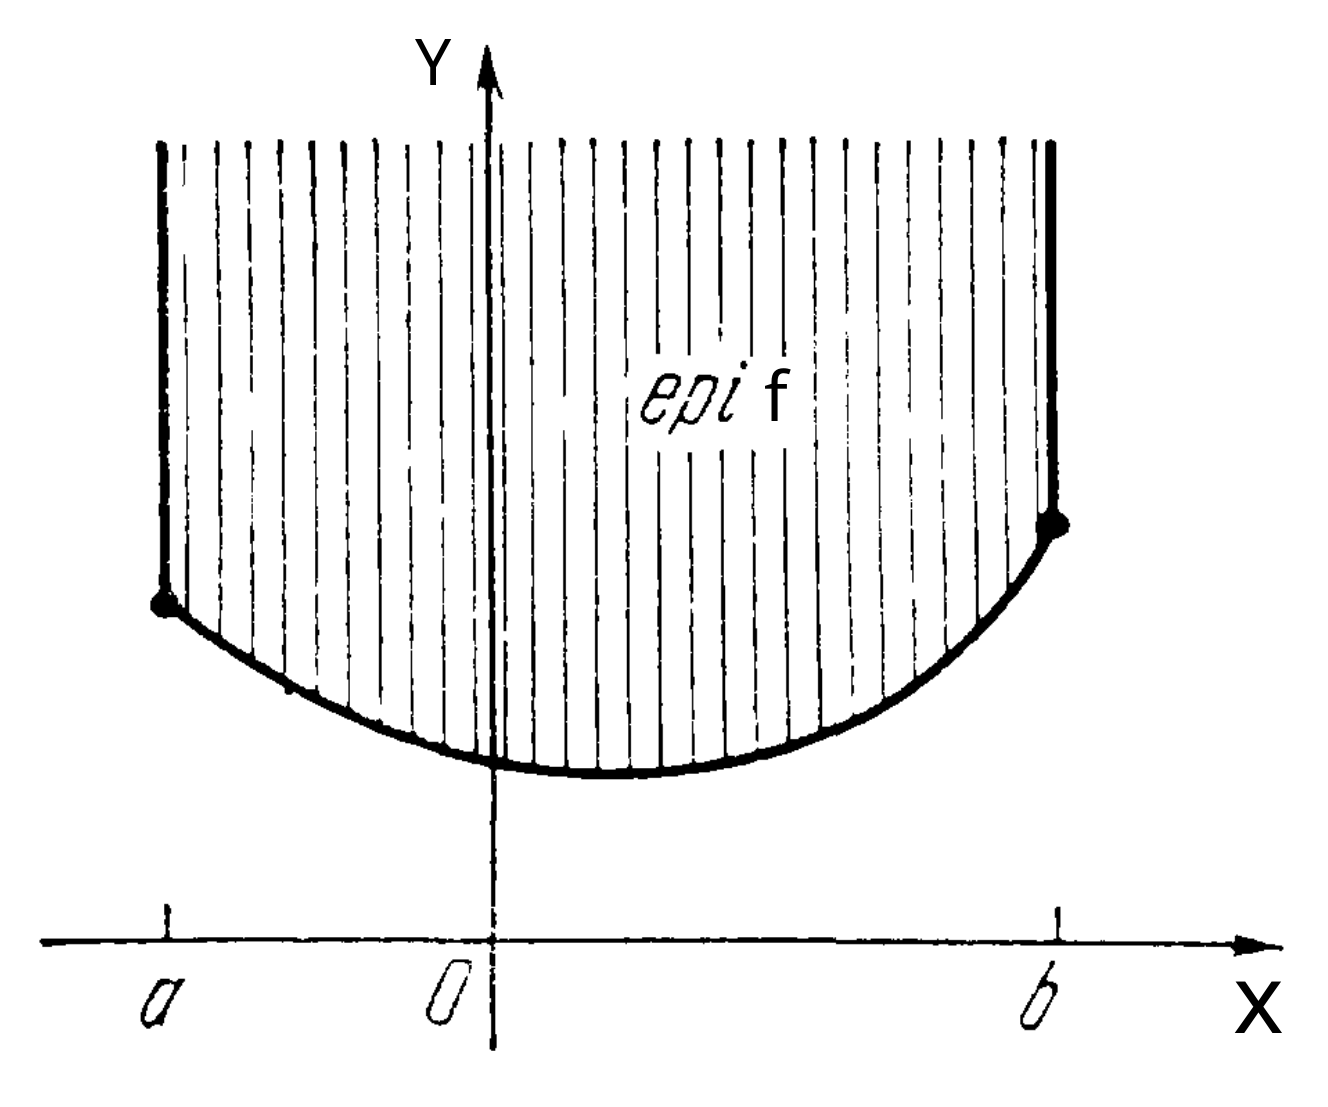
\includegraphics[width=.6\linewidth]{img/teor9}
	\caption{Надграфик}
	\label{fig:teor9}
	\end{figure}
\end{definition}
\end{multicols}

\begin{theorem}[Критерий выпуклости функции]
	Для того чтобы функция $f(x)$, определенная на выпуклом множестве $U$, была выпуклой на $U$, необходимо и достаточно, чтобы ее надграфик был выпуклым множеством.
	\begin{proof}
		Необходимость. Пусть функция $f(x)$ выпукла на выпуклом множестве $U$. Возьмем две произвольные точки $z_1=(x_1,\,y_1),\,z_2=(x_2,\,y_2)\in \operatorname{epi} f$ и составим их выпуклую комбинацию\footnote{Точка $z$ называется \textit{выпуклой комбинацией} точек $z_1,\,\dots,\,z_n$, если существуют числа $\alpha_1\geq0,\,\dots,\,\alpha_n\geq0$, $\sum_{i=1}^{n}\alpha_i = 1$ такие, что $z = \sum_{i=1}^{n}z_i\cdot\alpha_i$} $z_\alpha = \alpha z_1 + (1-\alpha)z_2 = (\alpha x_1 + (1-\alpha)x_2,\,\alpha y_1 + (1-\alpha)y_2)$, $(0\leq\alpha\leq1)$. Из выпуклости $U$ следует, что $\alpha x_1 + (1-\alpha)x_2 \in U$. Из выпуклости $f(x)$, учитывая, что $z_1,\,z_2\in\operatorname{epi}f$, имеем $f(z_\alpha) \leq \alpha f(x_1)+(1-\alpha)f(x_2)\leq\alpha y_1 + (1-\alpha)y_2$. Следовательно, $z_\alpha\in\operatorname{epi}f$ при всех $\alpha\in \left[0,\,1\right]$. Выпуклость $\operatorname{epi}f$ доказана.
		
		Достаточность. Пусть $\operatorname{epi}f$ -- выпуклое множество. Возьмем произвольные $x_1,\,x_2\in U$ и $\alpha\in\left[0,\,1\right]$. Тогда $z_1=(x_1,\,f(x_1)),\,z_2=(x_2,\,f(x_2))\in\operatorname{epi}f$. В силу выпуклости $\operatorname{epi}f$ точка $z_\alpha=\alpha z_1 + (1-\alpha)z_2\in\operatorname{epi}f$. Это значит, что $\alpha f(x_1) + (1-\alpha)f(x_1) \leq f\left(\alpha x_1 + (1-\alpha)x_2\right)$. Выпуклость $f(x)$ доказана.
	\end{proof}
\end{theorem}

